\chapter{A single step evolution model driven by digital Elastica minimization}
\label{chapter:balance-flow}


In this chapter we introduce the balance coefficient, a value that indicates how far the intersection of some disk and a digital shape is from half of the disk area. This value motivates the definition of a new family of energies to regularize the squared curvatute: the $m$-BalanceFlow. We are going to show that the BalanceFlow is closely related to the FlipFlow energy, but the former has an easier interpretation and a simpler algorithm to implement.


\section{Definitions}
In section \ref{sec:flipflow-algorithm-discussion}, we have argued that inverting the solution was necessary to reduce the squared curvature estimation in the next shape of the flow. In this section, we formalize the key concept involved in our argumentation.

\begin{definition}{Balance coefficent}
Given digital shape $S \in \Omega$, positive number $r$ and point $p \in \Omega$, the \emph{balance coefficient} of $S$ at $p$ is defined as

\begin{align*}
	u(S,p) = ( \frac{\pi r^2}{2} - |B_r(p) \cap S| )^2.
\end{align*}

\end{definition}

The balance coefficient definition is very similar to the II squared curvature estimator. Nonetheless, we have decided to make a new definition since we don't have the scaling factor $\frac{9}{R^6}$ and that the balance coefficient can be computed everywehere and not only in the digital boundary of the shape. Let $F=B_r(p) \cap S$ and $G=B_r(p) \setminus F$. The balance coefficient is symmetric with respect $F$ and $G$. 

\begin{align*}
	u(S,p) &= ( \frac{\pi r^2}{2} - |F| )^2 = ( -\frac{\pi r^2}{2} + |G| )^2 = ( \frac{\pi r^2}{2} - |G| )^2.
\end{align*}

The balance coefficient is used to estimate the effect of moving the estimation ball center towards the interior or the exterior of the shape. For example, consider the figure \ref{fig:balance-plot} in which we plot the balance coefficients of points along the diagonal of a square shape. 

\begin{figure}
\center
\begin{minipage}{0.25\textwidth}
\subfloat{
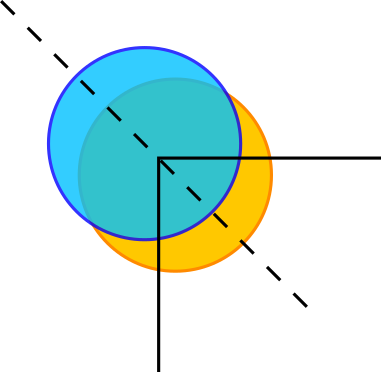
\includegraphics[scale=1.0]{figures/chapter7/distant-disks-1.png}}\\%
\subfloat{
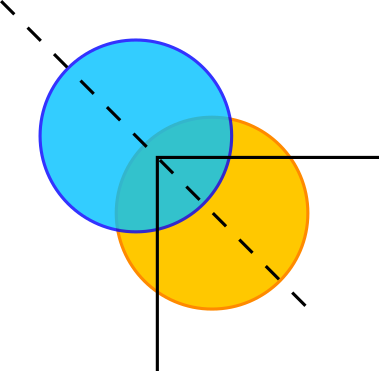
\includegraphics[scale=1.0]{figures/chapter7/distant-disks-2.png}}\\%
\subfloat{
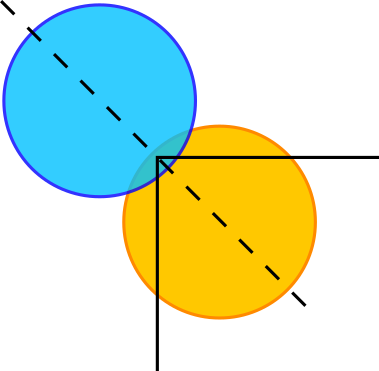
\includegraphics[scale=1.0]{figures/chapter7/distant-disks-3.png}}
\end{minipage}%
\begin{minipage}{0.75\textwidth}
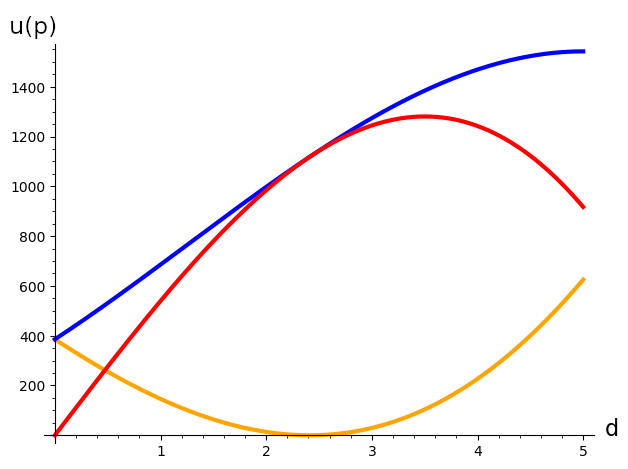
\includegraphics[scale=0.75]{figures/chapter7/balance-coefficient-p2-with-sum.png}
\end{minipage}
\caption{The balance coefficient of equidistant points from the shape contour. The red curve indicates the difference between the blue and the orange curve. The intersection point with the $x$-axes or the inflexion point in the red curve indicates the best center point for the estimation ball at the corner. }
\label{fig:balance-plot}
\end{figure}


The balance coefficient grows if the estimation ball is moved towards the exterior and decreases if the estimation ball is moved towards the interior of the shape. That is an indication that we should remove point $p$ from $S$ to decrease the squared curvature of the shape at point $p \in \partial S$. The same point $p$ may be touched by several balls, each of them contributing with some value for the ultimate decision of keep or remove point $p$ of $S$. 
%The $m$-balance is defined as the sum of these contributions


%\begin{definition}{m-balance}
%Given digital shape $S$, integer numbers $r>0, m \neq 0$, the \emph{m-balance} at point $p$ is defined as
%
%\begin{align*}
%	U_{m}(S,p) &= \sum_{q \in Q_m(p)}{ u(S,q)}
%\end{align*}
%
%where its zone of influence $Q_m(p)$ is defined as
%
%\begin{align*}
%	Q_m(p) &= \left\{\; q \in L_m(S) \; | \; p \in B_r(q) \; \right\} \\
%\end{align*}
%
%\end{definition}
%
%\begin{figure}[h!]
%\center
%\includegraphics[scale=0.5]{figures/chapter7/k-balance.png}
%\caption{The $q$ points of the $m$-ring forms the zone of influence of the boundary point $p$.}
%\label{fig:balance-set}
%\end{figure}
%
%The zone of influence of $p$ is the set of all points $q$ in which $p$ is contained in the estimation ball centered at $q$. In the next section we define a flow that will have the following behaviour
%
%\begin{align*}
%	U_m(S^{(k)},x_j) - U_{-m}(S^{(k)},x_j) > 0 &\rightarrow x_j \notin S^{(k+1)} \\
%	U_m(S^{(k)},x_j) - U_{-m}(S^{(k)},x_j) < 0 &\rightarrow x_j \in S^{(k+1)}
%\end{align*}



We are going to consider the inner and outer pixel boundary simultaneously as the optimization variables. We recall that $S^{(k)}$ corresponds to the digital shape $S$ after the $k$th iteration of the flow and that $d_{S^{(k)}}$ is its signed distance transform. We list the sets needed to define the new family of energies:

\begin{align*}
	O^{(k)} &:=\left\{ p \in \Omega \; | \; -1 <= d_{S^{(k)}}(p) \leq 1 \right\}\\
	X^{(k)} &:= X(O^{(k)})  \\
	F^{(k)} &:= S^{(k)} \setminus O^{(k)} \\
	F_r^{(k)}(p) &:= F^{(k)} \cap B_r(p)\\
	O_r^{(k)}(p) &:= O^{(k)} \cap B_r(p) \\
	X_r^{(k)}(p) &:= X\big( O_r^{(k)}(p) \big).
\end{align*}

We assume $k=0$ if not defined, i.e., $S=S^{(0)}$. We denote $p_i, p_o \in \mathcal{R}_m(S)$ as the inner and outer ball centers in the $m$-ring of $S$, respectively. To simplify notation, let $X_o=X_r(p_o)$ and $X_i=X_r(p_i)$. We define the term $T_{m}^{bal}(S)$ as

\begin{align}
	T_{m}^{bal}(S) &= \sum_{p_i,p_o \in \mathcal{R}_m(S)}{( \frac{\pi R^2}{2} - (\; |F_o| + \sum_{ x_j \in X_o}{1-x_j} \; ) )^2 -(\frac{\pi R^2}{2} - (\; |F_i| + \sum_{x_j \in X_i}{x_j}\;))^2}.
	\label{eq:balance-term}
\end{align}

Locally, labeling $x_j=0$ implies to change the initial balance of the outer ball, while keeping the initial balance of the inner ball unchanged. 

The $m$-balance energy family is defined as

\begin{align}
  E_{(\Theta,m)}^{bal}(X^{(k)},S^{(k)}) =& \sum_{x_j \in X^{(k)}}{\alpha s(x_j)} + \beta T_{m}^{bal}(S^{(k)}) + \sum_{x_j \in X^{(k)}}{\gamma g(S^{(k)},x_j)}.
  \label{eq:single-step-energy-family}
\end{align}

We follow the same notation of chapter \ref{chapter:flip-flow} to denote the data term $g(S,x)$ and the length penalization term $s(x)$ defined below. 

\begin{align}
  s(x_{w(p)})=\sum_{q \in \mathcal{N}_4(p)}{ t(q) }, \quad \text{where } t(q) = \left\{\begin{array}{ll}
  (x_{w(p)}-x_{w(q)})^2, & \text{if } q \in O^{(k)}\\
  (x_{w(p)}-1), & \text{if } q \in F^{(k)}\\
  (x_{w(p)}-0), & \text{otherwise }
  \end{array}\right.
  \label{eq:single-step-length-penalization}
\end{align}

\begin{align}
  g(x_{w(p)}) = -x_{w(p)}\log{H_f(p)} - (1-x_{w(p)})\log{H_b(p)},
  \label{eq:single-step-data-fidelity}
\end{align}	

where $H_f ,H_b $ are the mixed Gaussian distributions of color intensities derived from the foreground and background seeds. The BalanceFlow algorithm is summarized in \ref{alg:balance-flow} and an illustration is shown in figure \ref{fig:ch7-segmentation}.

\begin{algorithm}
 \SetKwData{It}{k}
 \SetKwData{MIt}{maxIt}
 \SetKwData{Delta}{delta}
 \SetKwInOut{Input}{input}\SetKwInOut{Output}{output}
 \SetKwComment{comment}{//}{}
 
 \Input{A digital set $S$; The ring number $m$; parameter vector $\Theta=\alpha,\beta)$; data term coefficient $\gamma$; the maximum number of iterations \MIt;}
 \BlankLine
 $S^{(0)} \longleftarrow S$\;
 $k \longleftarrow 1$\;
 \While{ \It $<$ \MIt  }{ 	
	 	$x^{(k-1)} \longleftarrow \argmin_{X^{(k-1)}} E_{(\Theta,m)}^{bal}(X^{(k-1)},S^{(k-1)}) + \gamma g(X^{(k-1)})$\; 	
 		$S^{(k)} \longleftarrow F^{(k-1)} + x^{(k-1)}$\;
 	
	\It $\longleftarrow$ \It $+1$\;
	
 }
 \caption{BalanceFlow algorithm.}
 \label{alg:balance-flow}  
\end{algorithm}

\begin{figure}
\center
\begin{tabular}{cccc}
\multirow{2}{*}{Seeds} & \multirow{2}{*}{GrabCut} & $\alpha=0.5, \beta=0.0,$ & $\alpha=0.5, \beta=1.0,$\\
& & $\gamma=2.0$ & $\gamma=2.0$\\
 	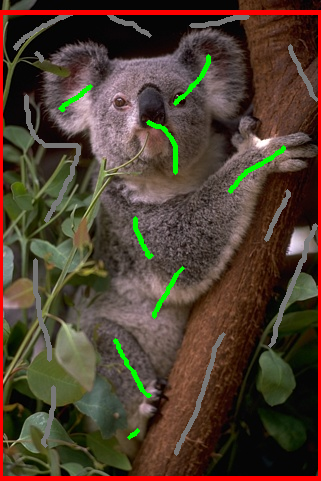
\includegraphics[scale=0.25]{figures/chapter7/segmentation/coala/k-0.0/seeds.png} & 
 	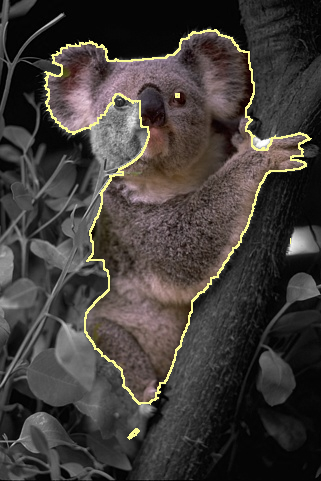
\includegraphics[scale=0.25]{figures/chapter7/segmentation/coala/k-0.0/gc-seg.png} &  	
 	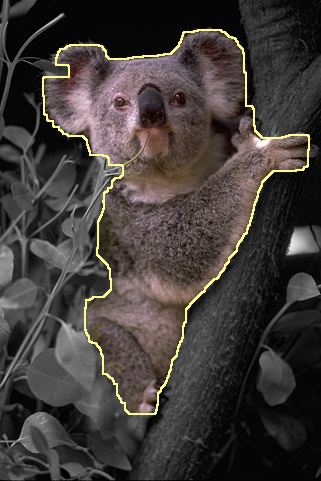
\includegraphics[scale=0.25]{figures/chapter7/segmentation/coala/k-0.0/corrected-seg.png} &  	
 	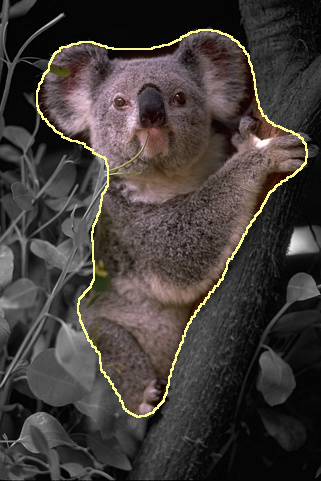
\includegraphics[scale=0.25]{figures/chapter7/segmentation/coala/k-1.0/corrected-seg.png}
\end{tabular}	
\caption{Given foreground (green) and background (gray) seeds at picture (a); GrabCut produces picture (b) which is used as input of the BalnceFlow Contour Correction algorithm; in pictures (c) and (d) we display the output of Contour Correction algorithm with and without squared curvature regularization. }
\label{fig:ch7-segmentation}
\end{figure}


\section{Relation with FlipFlow}
	The BalanceFlow returns similar solutions to the FlipFlow algorithm. Indeed, they are closely related. We recall the curvature regularization term of the FlipFlow energy \eqref{eq:energy-family} for some digital shape $S$ before proving proposition

\begin{align}
T_{m}^{flip}(S) &= \sum_{ p_i,p_o \in R_m(S)}{ ( \frac{\pi R^2}{2} - F_r(p_o) - \sum_{x_j \in X_r(p_o)}{x_j})^2 + (\frac{\pi R^2}{2} - F_r(p_i) - \sum_{x_j \in X_r(p_i)}{x_j})^2 }
\label{eq:curvature-term}
\end{align}

\begin{proposition}{FlipFlow and BalanceFlow relation}
The curvature terms of FlipFlow and BalanceFlow are related by the equality
\begin{align*}
T_{m}^{flip}(S) &= T_{m}^{bal}(S) + P_1(X_i) + c,
\end{align*}
where $P_1(X_i) = (\sum_{X_i}{ 1-x_j})^2 + (\sum_{X_i}{x_j})^2.$
\label{prop:flipflow-balanceflow-relation}
\end{proposition}

\begin{proof}

We start by replacing $x_j$ to $(1-x_j)$ in \eqref{eq:curvature-term}, which corresponds to take the complement of the solution in the FlipFlow model. To simplify notation, we are going to ommit the radius $r$ and replace points $p_i,p_o$ by an underscored $i,o$, i.e., $F_i := F_r(p_i)$. We rewrite \eqref{eq:curvature-term} as

\begin{align}
T_{m}^{flip}(S) &= \sum_{ p_i,p_o \in R_m(S)}{ ( \frac{\pi R^2}{2} - F_o - \sum_{x_j \in X_o}{1-x_j})^2 + (\frac{\pi R^2}{2} - F_i - \sum_{x_j \in X_i}{1-x_j})^2 }
\label{eq:curvature-term-simplification}
\end{align}

Next, let $A_i = \pi R^2/2 - |F_i|$. We rewrite  the second term of \eqref{eq:curvature-term-simplification} as

\begin{align*}
	\Big(A_i - \sum_{x_j \in X_i}{ (1-x_j) } \Big)^2 &= \Big( A_i - |X_i| + \sum_{x_j \in X_i}{ x_j } \Big)^2 \\
	&= (A_i - |X_i|)^2 + 2(A_i - |X_i|)\sum_{x_j \in X_i}{x_j} + \Big( \sum_{x_j \in X_i}{x_j} \Big)^2\\	
	&= A_i^2 -2A_i|X_i| + |X_i|^2 + 2(A_i - |X_i|)\sum_{x_j \in X_i}{x_j} + \Big( \sum_{x_j \in X_i}{x_j} \Big)^2\\
	&= A_i^2 + 2A_i\sum_{x_j \in X_i}{x_j} + \Big( \sum_{x_j \in X_i}{x_j} \Big)^2 - 2A_i|X_i| + |X_i|^2 -2|X_i|\sum_{x_j \in X_i}{x_j} \\
	&= 2A_i^2 - \Big(A_i - \sum_{x_j \in X_i}{x_j}\Big)^2 + 2\Big( \sum_{x_j \in X_i}{x_j} \Big) ^2 - 2A_i|X_i| + |X_i|^2 - 2|X_i|\sum_{x_j \in X_i}{x_j}
\end{align*}

	We group the constants into the constant term $c=2A_i^2 - 2A_i|X_i|$	 to obtain
\begin{align}
		\Big(A_i - \sum_{x_j \in X_i}{ (1-x_j) }\Big)^2 &= - \Big(A_i - \sum_{}{x_j}\Big)^2 + \Big(|X_i| - \sum_{x_j \in X_i}{x_j}\Big)^2 + \Big(\sum_{x_j \in X_i}{x_j}\Big)^2 + c \nonumber \\
	&= - \Big(A_i - \sum_{x_j \in X_i}{x_j}\Big)^2 + P_1(X_i) + c \nonumber \\
	&= - \Big(\frac{\pi R^2}{2} - (|F_i| + \sum_{x_j \in X_i}{x_j}) \Big)^2 + P_1(X_i) + c \nonumber 	
	\label{eq:second-term}
\end{align}

Finnaly, we  replace \eqref{eq:second-term} in \eqref{eq:curvature-term-simplification} to obtain

\begin{align}
T_{m}^{flip}(S) &= ( \frac{\pi R^2}{2} - (\; |F_o| + \sum_{ x_j \in X_o}{1-x_j} \; ) )^2 -(\frac{\pi R^2}{2} - (\; |F_i| + \sum_{x_j \in X_i}{x_j}\;))^2  + P_1(X_i) + c \nonumber \\
&= T_{m}^{bal}(S) + P_1(X_i) + c.
\end{align}

\end{proof}

Proposition \ref{prop:flipflow-balanceflow-relation} tell us that, apart  from a constant, the two energies differ in the penalty term $P_1(X_i)$. Locally, such term favors solutions in which half of the variables touched by the inner ball are labeled one. Indeed, the FlipFlow and BalanceFlow behave similarly. In the next chapter we make extensive comparisons between them.

%\begin{figure}
%\begin{tabular}{cccc}
%$7$-BalanceFlow & 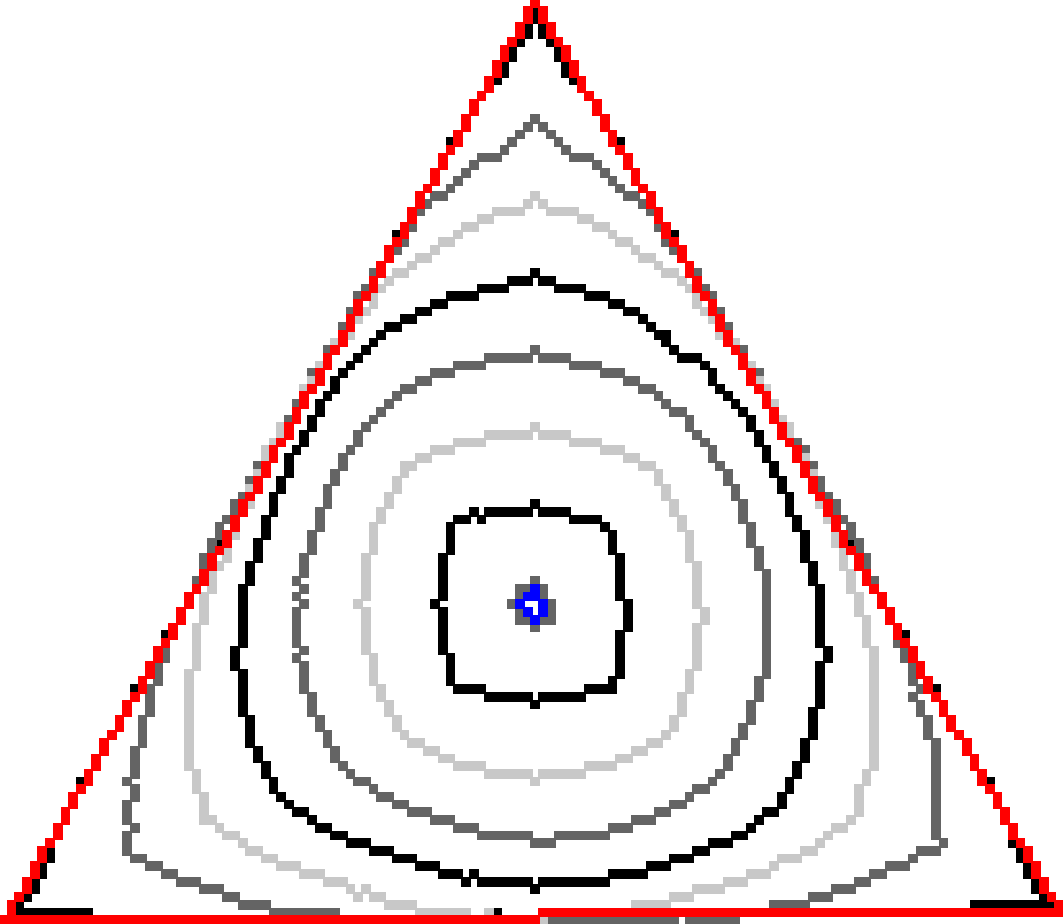
\includegraphics[scale=0.25]{figures/chapter7/balance-flow/triangle/summary.pdf} & 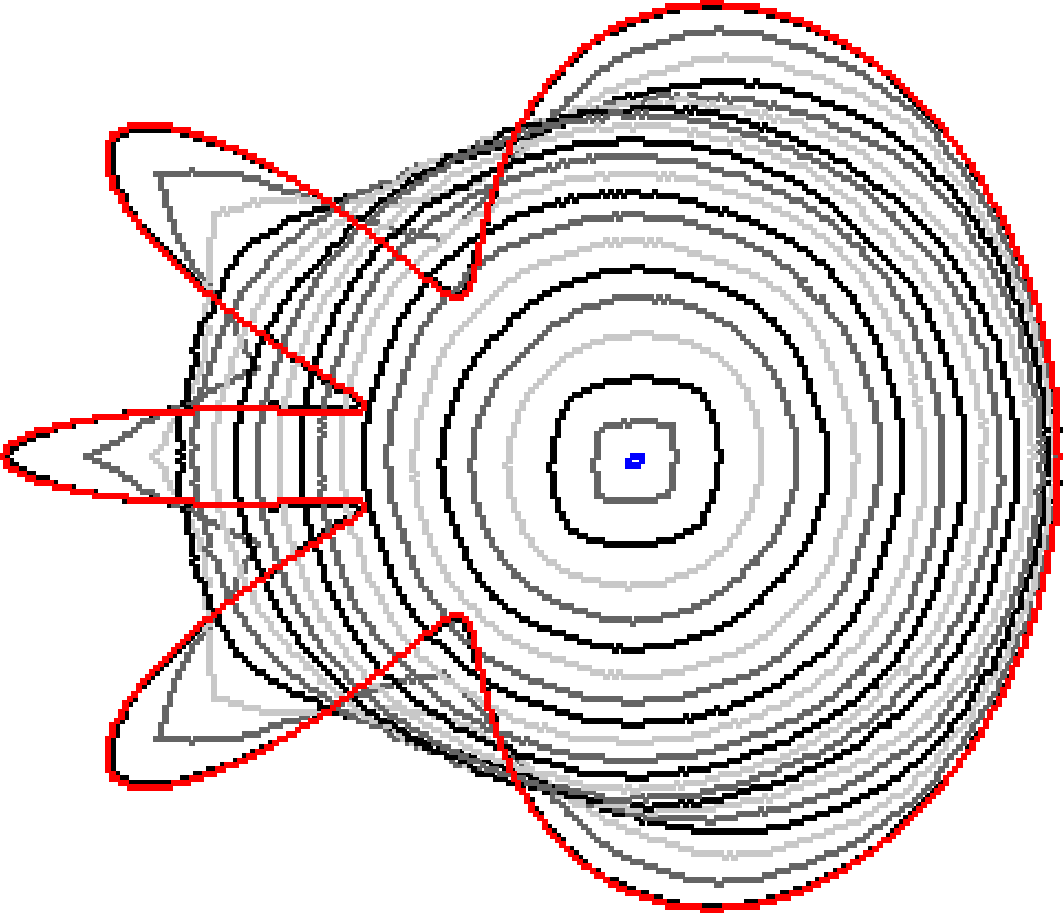
\includegraphics[scale=0.25]{figures/chapter7/balance-flow/flower/summary.pdf} & 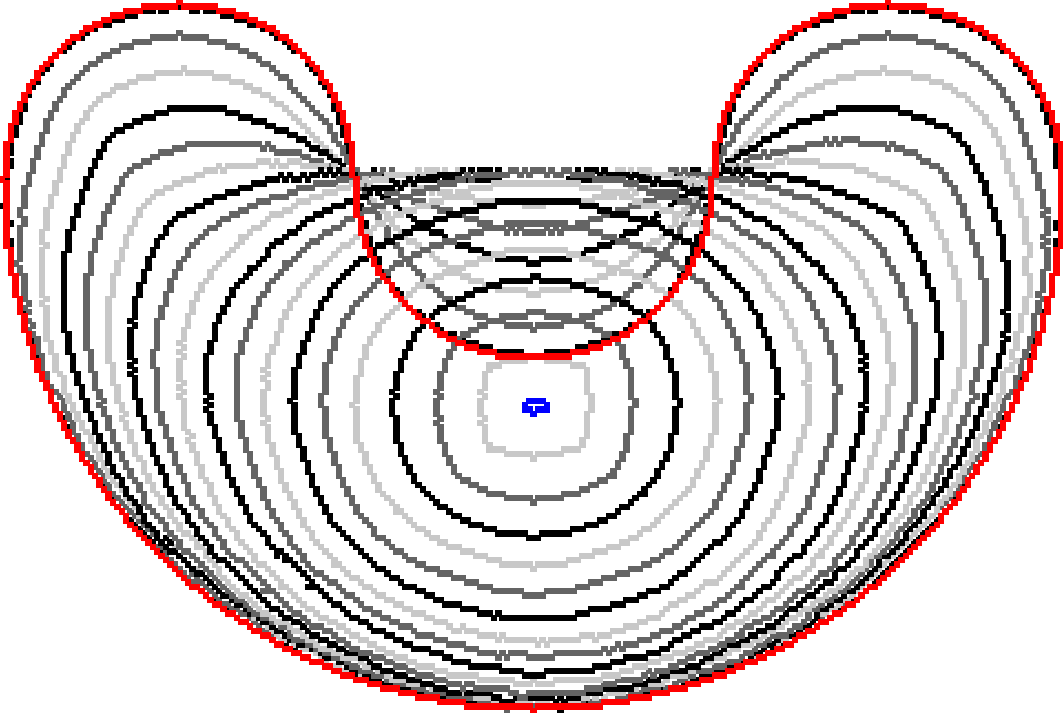
\includegraphics[scale=0.25]{figures/chapter7/balance-flow/bean/summary.pdf} \\
%$7$-FlipFlow & 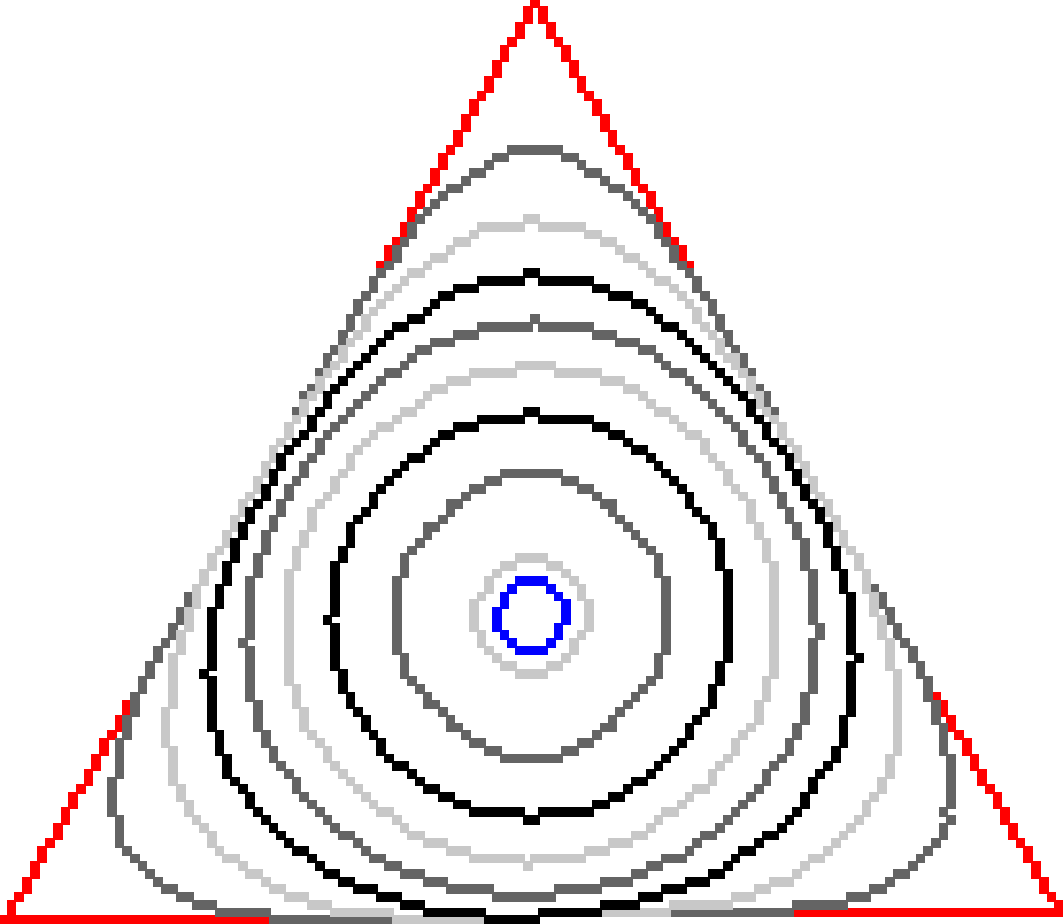
\includegraphics[scale=0.25]{figures/chapter7/flip-flow/triangle/summary.pdf} & 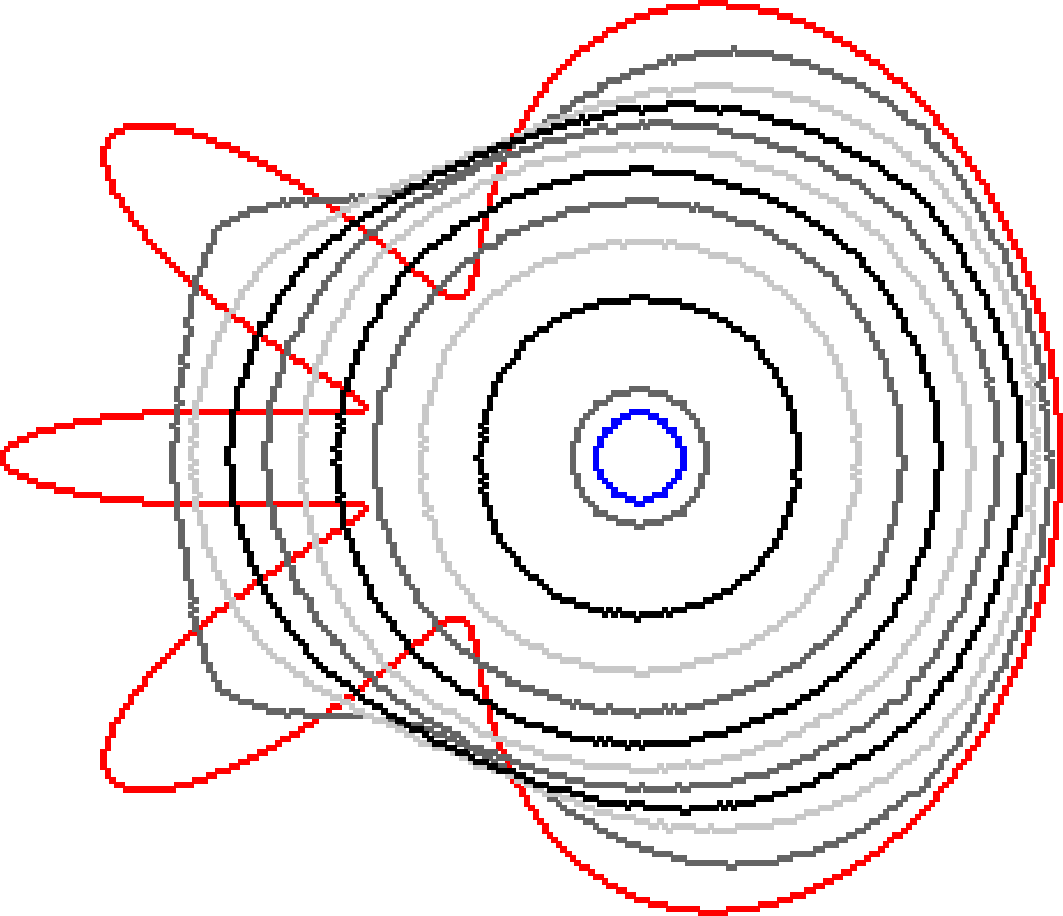
\includegraphics[scale=0.25]{figures/chapter7/flip-flow/flower/summary.pdf} & 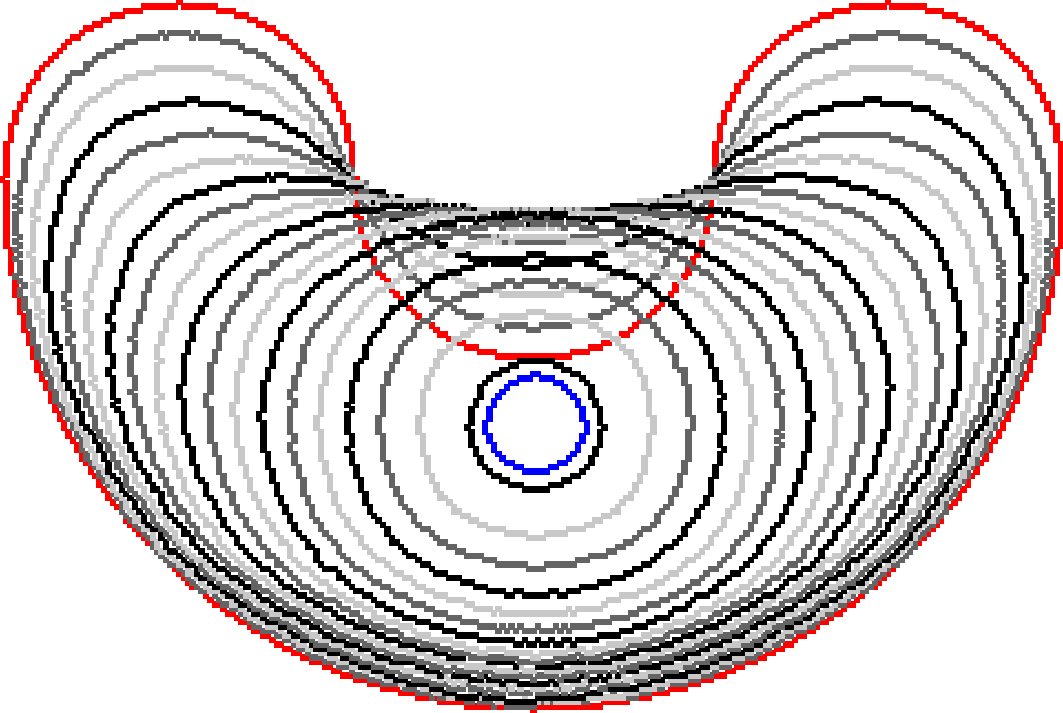
\includegraphics[scale=0.25]{figures/chapter7/flip-flow/bean/summary.pdf} \\
%\end{tabular}
%\caption{Evolutions of three shapes for the $7$-BalanceFlow and $7$-FlipFlow using a estimation ball radius of $9$. The models present similiar behaviour. Shapes are displayed at every $10$ iterations.}
%\label{fig:balance-flow-flip-flow-comparison}
%\end{figure}

\section{Towards a graph-based formulation}

Let $A_o = \pi R^2 / 2 - |F_o|$ and $A_i = \pi R^2/2 - |F_i|$. Putting $x_j$ in evidence we can rewrite \eqref{eq:balance-term} as

\begin{align*}
	T_{m}^{bal}(S) &= \Big(A_o - |X_o| + \sum_{x_j \in X_o}{x_j} \Big)^2 - \Big(A_i - \sum_{x_j \in X_i}{x_j}\Big)^2 \\
	&= (A_o - |X_o|)^2 - A_i^2 + 2(A_o - |X_o|)\sum_{x_j \in X_o}{x_j} + 2A_i\sum_{x_j \in X_i}{x_j} + \sum_{x_j \in X_o}{x_j}^2 - \sum_{x_j \in X_i}{x_j}^2.
\end{align*} 

Grouping the constants in $c=(A_o - |X_o|)^2 - A_i^2$ and putting $x_j$ in evidence we obtain

\begin{align}
	T_{m}^{bal}(S) 	&= c +\sum_{x_j \in X}{ 2x_j\Big( A_o - |X_o| + \frac{1}{2}\sum_{x_l \in X_o}{x_l} + A_i - \frac{1}{2}\sum_{x_l \in X_i}{x_l}\Big)} \nonumber \\
	&= c +\sum_{x_j \in X}{2x_j\Bigg( \Big(A_o - \sum_{x_l \in X_o}{1-\frac{x_l}{2}}\Big) + \Big(A_i - \sum_{x_l \in X_i}{\frac{x_l}{2}}\Big)\Bigg)}.
	\label{eq:xj-evidence}
\end{align}

We remark the similarity of the expression between parentheses in \eqref{eq:xj-evidence} and the sum $u(S,p_o)^{1/2} + u(S,p_i)^{1/2}$, i.e., the sum of balance coefficients square roots. The variable $x_j$ is set to zero if the expression in parentheses is less than zero. That remark motivates us to define a graph-based model, described in the next chapter, in which the edge's weight are given by the sum of balance coefficients.


\section{Conclusion}
The BalanceFlow model is closely related to the FlipFlow but it has a simple implementation and interpretation. The balance coefficent is the link that connects both models and the motivation for the graph-based model proposed in the next chapter.




